\documentclass{article}
\usepackage[left=2cm, right=2cm, top=0cm]{geometry}
\usepackage{amsmath}
\usepackage{amssymb}
\usepackage{graphicx}
\usepackage{tikz}
\usepackage{enumitem}
\usepackage[margin=2cm]{caption}
\usepackage{hyperref}

\setlength\parindent{0pt}
\hypersetup{
    colorlinks,
    citecolor=green,
    filecolor=black,
    linkcolor=blue,
    urlcolor=blue
}

\begin{document}
\title{Assignment 2}
\author{Jacob Puthipiroj}
% \date{}
\maketitle

\makeatletter
\newcommand{\mybox}{%
    \collectbox{%
        \setlength{\fboxsep}{1pt}%
        \fbox{\BOXCONTENT}%
    }%
}


\section*{Nagel-Schrenkerg (Single Lane) Models }


Cellular Automata models of traffic flow began with the work of Nagel and Schrenkenberg (1992). In the Nagel-Schrenkenberg model, the road is divided into cells, each possibly containing a maximum of one car. To model a circular road, the boundaries are considered periodic; cars exiting the road on the right automatically reenter the space on the left. Furthermore, time is discretized into steps, and at each time step, cars follow an update rule:
\begin{enumerate}[itemsep=0.1pt]
\item \textbf{Acceleration:} If the car is not at its maximum velocity, increase its velocity by one.
\item \textbf{Deceleration:} If the distance to the car in front is less than the current car's velocity, decrease the speed to exactly the distance to the car in front to avoid a collision.
\item \textbf{Randomized Slowdown:} If the car is not static, reduce their velocity by 1 with probability $p$. This is to model random behaviors on roads, such as hard braking.
\item \textbf{Motion}: The cars now move according to their new probabilities.
\end{enumerate}
By convention, states of cars on the road are displayed between steps 3 and 4. An example is shown below. 

\begin{figure}[h]
\begin{minipage}[t]{.5\textwidth}
\raggedright
......5........5..............5.................................................
...........5........4..............5............................................
................5.......4...............5.......................................
.....................5......5................4..................................
..........................4......4...............5..............................
..............................4......5................5.........................
..................................5.......5................4....................
.......................................5.......5...............5................
............................................4.......5...............4...........
................................................5........4..............4.......
.....................................................4.......4..............5...
.4.......................................................4.......4..............
.....5.......................................................5.......4..........
..........4.......................................................5......5......
..............5........................................................5......5.
...4...............5........................................................4...
4......4................4.......................................................
....5......4................4...................................................
\end{minipage}% <---------------- Note the use of "%"
\begin{minipage}[t]{.5\textwidth}
\raggedleft
........5.....0.0.5.............5.............04...............2..4.............
.............01.0......5.............5........0....5.............2....5.........
.............0.01...........4.............2...1.........5..........2.......4....
.............1.0.2..............4...........2..2.............4.......2.........4
...4..........00...2................4.........1..3...............5.....3........
.......4......01.....2..................5......2....4.................3...4.....
...........2..1.1......3.....................2...3......5................3....5.
...5.........0.1.2........3....................3....4........5..............4...
4.......3....1..1..2.........4....................3.....4.........4.............
....5......1..2..1...2...........5...................3......5.........5.........
.........2..1...1.1....2..............4.................3........5.........4....
...........1.2...0.2.....3................4................4..........5........5
....5.......1..0.0...2......3.................5................5...........4....
.........2...0.1.1.....3.......3...................4................4..........5
....5......0.1..1.1.......3.......4....................4................5.......
.........1.0..1..0.1.........3........5....................5.................5..
..5.......01...1.0..1...........3..........4....................4...............
.......2..0.1...01...2.............3...........4....................4...........

\end{minipage}

\caption{Both figures show cellular automata simulations with a periodic (circular) road of length 80, a maximum velocity of 5, and $p = 0.5$. While cars slow down randomly. on the left, the sparsity of the open road (0.03) prevents a traffic jam from forming. On the right, with identical parameters but on a denser road (0.1), cars within the jam slow down and prevent the jam from clearing. Instead, the jam slowly moves left throughout the simulation.}
\end{figure}

Nagel and Schrenkenberg used flow ---defined as the number of vehicles passing a reference point per unit of time--- to compare between various cellular automata models. Intuitively, a model with a very high density should have roads so congested that few cars can move freely through the reference point, and thus have low flow, while models with too low a density should also have very few cars moving through the point. Thus the density of maximum flow should lie somewhere in between.

\newgeometry{left=2cm, right=2cm}
\begin{figure*}
\centering
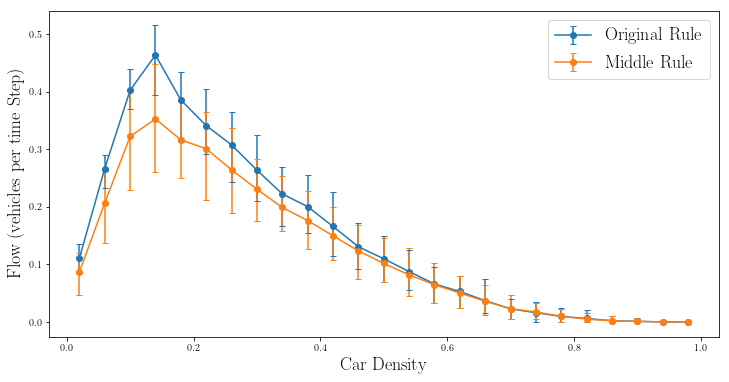
\includegraphics[scale = 0.6]{middleorig.png}
\caption{This shows cellular automata simulations with a length of 100, a maximum velocity of 5, $p = 0.2$, Flow, as a function of car density follows an inverted V shape, peaking sharply at a density of around 0.15, before gradually becoming less efficient. When cars follow the 'always in the middle' rule, flow are generally less efficient.}
\end{figure*}
%We are citing \cite{nagel1992cellular}.

%	Over time, we see that traffic jams can appear with sufficient traffic density. However, depending on the rule of the model, these can eventually disappear.

A further augmentation of the algorithm is for cars in the model to aim to be around the same distance from the car in front as to the car in the back. This is slightly more complicated, but yields better flow results, and is as follows:
\begin{enumerate}[itemsep=0.1pt]
\item \textbf{Acceleration/Deceleration:} Check the distance to the car in front, and to the car at the back. \begin{enumerate}
\item If the distance to the car in front is greater than the distance to the car in the back, accelerate the car by one if the car is not already at the maximum speed, and if the car will not exceed the distance to the car in front.
\item Otherwise, reduce the speed by one if the car is not already static, or reduce the speed to the distance to the car in front, whichever is less.
\end{enumerate}

\end{enumerate}


%When using the 'always in the middle' rule, we see that with up to 50\% traffic density, jams eventually disappear. 

%Try to look for the relationship between pslow, density, and max speed. 

%Following the Nagel-Schrenkberg model (1992), we see... 

\newpage
\section*{Rickert (Multi-Lane) Models}

In this section, we implement Rickert's (1996) extension to the Nagel-Schrankenberg model. Rickert allows for multiple lanes in the cellular automata model, and adds the ability for cars to switch lanes. The new algorithm sequence is thus: 
\begin{enumerate}
\item \textbf{Switch Lanes:} If the distance to the car in front is less than the car's current velocity, then consider switching. Otherwise, there is no need to switch and continue to step 2.
\begin{enumerate}
	\item Consider the lane to the left (if it exists). Otherwise, consider the right lane.
	\begin{enumerate}
	\item Calculate the distance to the front car, and to the back car.
	\item If the distance to the front is less than the current velocity \textbf{and} the distance to the back to less than the maximum velocity, switch to other lane.
	\end{enumerate}
	\item If a switch has been made, move on to step 2. Otherwise, consider the right lane if it exists and has not already been considered.
\end{enumerate}
\item \textbf{Accelerate/Decelerate:} Either following the original rule, or the 'always in the middle' rule.
\item \textbf{Randomized Slowdown:} Same as in the original model.
\item \textbf{Motion:} Same as in the original model. 
\end{enumerate}

\begin{figure}[h]
\centering
\begin{minipage}[t]{.5\textwidth}
\raggedright
...................5.5....5............5..............5.....5.....5........
..............5...........55.......5.....5.5................5.5..5.........
\

..................4.....3.....4............4.....................5.....5...
.......................4..0.....5.......5.1....4..........4..1..2....4.....
\

.5....................4.....4......5...........4..............4......4.....
.........................2.1.........5..0...2......4...........2...3.....4.

.....4....................4.....4......4...........4..............4.......5
..4......................0...2........1..1....2........4..........3...3....

....5.....5...................4.....4.......5...........5..............5...
......4...................1.....3.......2..2....2...........5.......2.....4

.5......4.....4...................4......5......4............5.............
...4......4................1.......3......2...3...2.............4.....2....

.....4.......5....4....................5......5......5...........4.........
.......4.......5............1.........3.....2...2....3..............4....3.

..........5......4....4.....................5.....4.......5..........4.....
..4.........5.......5........1...........3....2....3.....4..............4..



\end{minipage}% <---------------- Note the use of "%"
\begin{minipage}[t]{.5\textwidth}
\raggedleft
..5..5.......5.5...5.55...5....55...5..55.....5.5.5...5.5...55....5....55..
.......5..5...55..5..5....555.5....5.5...5.5.5.........55..5555..5......5..

.4.......4...0...2.0.0...3....40..2...20.....5.1....4.0....30....4...3.0...
3.....4..2..2.0.1..1.....400.1....4.1..2..10.....4....40.1.000.1.....4.....

.....4.....2.0....10..1.....3.0.1...2.00......1.1...0..1...00......2..1.1..
....4...2.1..1.1..2..2...000...2..0...2.1.00........3.0.10.00.1..2.......4.

.........4.0..1...0.1..1....0.0..1..0.0.1.....0...2..1...2.00........2....2
...5..2.0..1.0...2.1....300.1....20....10.0.1.......0..10.100..1...2....2..

..3.....2.10....2.0..1...2...10...1.0.0...2...0........2.0.00...........3..
.......4.1.0.0....1..2..00.1.1...00....00.0..1....0.0..0.1000....2...2....2

3....3...100.....10....2....30.1..0.0..1....2..1........1.10.1.............
..3.....10..1.1....1...200.0...2.00....00..1..1...0.0..0.0000......2....3..

...3....3000.....0.1.....2..0.1.1.0.0...1.....2.1.......0.00...2...........
3.....4.0.1..1.1....1..00.1.1...100....00...1..1...1.1..10000........2.....

.......40000.....0..1.....1.0.0..10.0....1....0...2......100......3........
...3..0..1.1.0...2....200..1.1..00.1...0.1....2.1..0..1.00000...........3..
\end{minipage}

\caption{Both figures show cellular automata simulations with a periodic (circular) road of length 80, a maximum velocity of 5, and $p = 0.5$. There are two lanes. Density on the left is $0.1$, and 0.4 on the right.}
\end{figure}










\newpage

\section*{Model Comparison}
When running 100 simulations at each of the densities tested, it does not actually seem like increasing the number of lanes actually helps to increase or decrease the mean flow rate. However, there is a considerable difference between their standard deviations. Based on the plot, we can see that a model with 4 lanes has the narrowest 95\% interval.\\

\begin{figure*}[h]
\centering
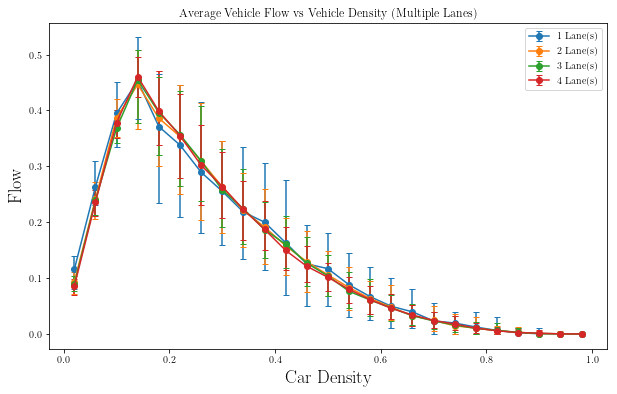
\includegraphics[scale = 0.6]{multilanemultiflow.png}
\caption{This shows cellular automata simulations with a length of 100, a maximum velocity of 5, $p = 0.2$, on various densities. It would seem that the number of lanes is inversely proportional to the width of the confidence interval. Thus while at the same density, a road with fewer lanes is more likely to 'get lucky' and achieve a higher flow rate, it is also more likely to be unlucky and achieve a lower flow as well.}
\end{figure*}

This model certainly has its limitations. However, it is possible to conceive of cases where the model might be somewhat useful. For example, on a wide open street, such as the 9 de Julio Avenue, there are up to 7 lanes in each direction, and cars rarely have to stop for other cars. During rush hour, large sections of the road which do not intersection with orthogonal streets could also be modeled with the multi-lane simulation. \\


There are behaviors encoded in the model which are slightly unrealistic - for example, every car on the model in actuality is trying (imperfectly, of course) to keep track of the cars in their vicinity, and adjust their speed accordingly. For example, 2 cars traveling at a speed of 5 could be less than 5 units apart, since both are reasonably certain that the other will not be hard-braking and suddenly stopping. Also, when deciding to switch lanes, cars do not necessarily leave 5 spaces between the lane to be switched to and the car behind them, for the same reason.\\

\section*{Future Work}
There are many features of road traffic that could have been included to make the model more realistic. The obstacles, speed-limit zones, and traffic lights for example would heavily increase the versatility of the model. We could have also included bad driver behavior, such as not flashing their lights, or honking their horn, or even drunk driving (which would cause a crash with some probability, or even get pulled over by a police car with some probability). Crashes are a part of modern traffic that would also greatly increase the realism of our model. 

\section*{Appendix}

\subsection*{Single Lane Traffic Flow}
The code used in this section is available \href{https://github.com/thetruejacob/CS166/blob/master/Nagel-Schrankenberg%20Model.ipynb}{here}.\\

\subsection*{MultiLane Traffic Flow}
The code used in this section is available \href{https://github.com/thetruejacob/CS166/blob/master/Rickert%20Model.ipynb}{here}.



\end{document}